% Template for Carleton problem sets
% Author: Andrew Gainer-Dewar, 2013
% This work is licensed under the Creative Commons Attribution 4.0 International License.
% To view a copy of this license, visit http://creativecommons.org/licenses/by/4.0/ or send a letter to Creative Commons, 444 Castro Street, Suite 900, Mountain View, California, 94041, USA.
\documentclass[twoside]{article}
\usepackage{ccpset}

% The Latin Modern font is a modernized replacement for the classic
% Computer Modern. Feel free to replace this with a different font package.
\usepackage{lmodern}

\title{EE445L - Lab04 Report}
\author{Kevin Gilbert\\ Gilberto Rodriguez}
\date{February 21, 2014}
\prof{Professor Bard}
\course{Lab: Monday/Wednesday 5-6:15}
\begin{document}
\maketitle{}

\section*{Requiremetns Document}
\subsection*{Overview}
\subsubsection*{Objectives}
The objectives of this project are to design, build and test a stepper motor controller. Educationally, students are learning how to interface a stepper motor, how to design with finite state machines, and how to perform state machine input/output in the background.
\subsubsection*{Process}
The project will be developed using the LM3S1968 board. There will be three switches that the operator will use to control the motor. The system will be built on a solderless breadboard and run on the usual USB power. The system may use the on board switches or off-board switches. A hardware/software interface will be designed that allows software to control the stepper motor. There will be at least three hardware/software modules: switch input, motor output, and the finite state machine. The process will be to design and test each module independently from the other modules. After each module is tested, the system will be built and tested.
\subsubsection*{Roles and Responsibilities}
EE445L students are the engineers and the TA is the client. Students are expected to make minor modifications to this document in order to clarify exactly what they plan to build. Students are allowed to divide responsibilities of the project however they wish, but, at the time of demonstration, both students are expected to understand all aspects of the design.
\subsubsection*{Interactions with Existing Systems}
The system will use the LM3S1968 board, a solderless breadboard, and the stepper motor. The wiring connector for the stepper motor is described in the PCB Artist file Lab4\_Artist.sch. It will be powered using the USB cable. You may use a +5V power from the lab bench, but please do not power the motors with a voltage above +5V.
\subsubsection*{Terminology}
\begin{itemize}
\item{Moore - a FSM where the output is only a fuction of the state and the next state is a function of the input and state}
\item{abstraction - the act of considering something as a general quality or characteristic, apart from concrete realities, specific objects, or actual instances} 
\item{board support package - a set of software routines that abstract the I/O hardware such that the same high-level code can run on multiple computers} 
\item{back emf - an electromagnetic force appearing in an inductive circuit in such a direction as to oppose any change of current in the circuit} 
\item{holding torque - the force times distance that the motor will remain stopped when its input pattern is constant}
\item{jerk - the change in acceleration or the derivative of the acceleration}
\item{full step - defined as the change occurring after one output using the full step sequence \{5,6,10,9\}} 
\item{CW - stands for clockwise} 
\item{CCW - stands for counterclockwise}
\end{itemize}
\subsubsection*{Security}
The system may include software from StellarisWare and from the book. No software written for this project may be transmitted, viewed, or communicated with any other EE445L student past, present, or future (other than the lab partner of course). It is the responsibility of the team to keep its EE445L lab solutions secure.
\subsection*{Function Description}
\subsubsection*{Functionality}
If all buttons are released, then the motor should stop. If switch 1 is pressed, spin at 4.2 revolutions per second in one direction as long as switch 1 continues to be pressed. If switch 2 is pressed, spin at 4.2 revolutions per sectond in the other direction as long as switch 2 continues to be pressed. If switch 1 and 2 are both pressed, the motor should continuously oscillate as fast as possible back and forth. The amplitude of this oscillation will be 8 steps. In other words, output the sequence \{CW, CW, CW, CW, CW, CW, CW, CW, CCW, CCW, CCW, CCW, CCW, CCW, CCW, CCW\} over and over as long as both switch 1 and 2 continue to be pressed and oscillates at 96Hz. If switch 3 is pressed then released, then step once in the CW direction. Any other combination (e.g., 1+3, 2+3, 1+2+3) should be ignored. You may assume the operator (you or the TA) will release the switches when it reaches the end of the worm gear. There will be a 1-1 mapping from the FSM graph and the C data structure. There is a delay for each state, which is saved in the FSM structure. The motor output is always one of these values 5, 6, 10, or 9. The motor moves such that the output never skips from 5 to 10, 10 to 5, 6 to 9, or 9 to 6. There are 23 states shown in the figure below. The FSM runs in the background using periodic interrupts. The foreground (main) initializes the FSM, then executes for(;;)\{\} do nothing loop. The maximum time to execute one instance of the ISR is 19.7 $\mu$seconds.
\vskip 0.1in
\centerline{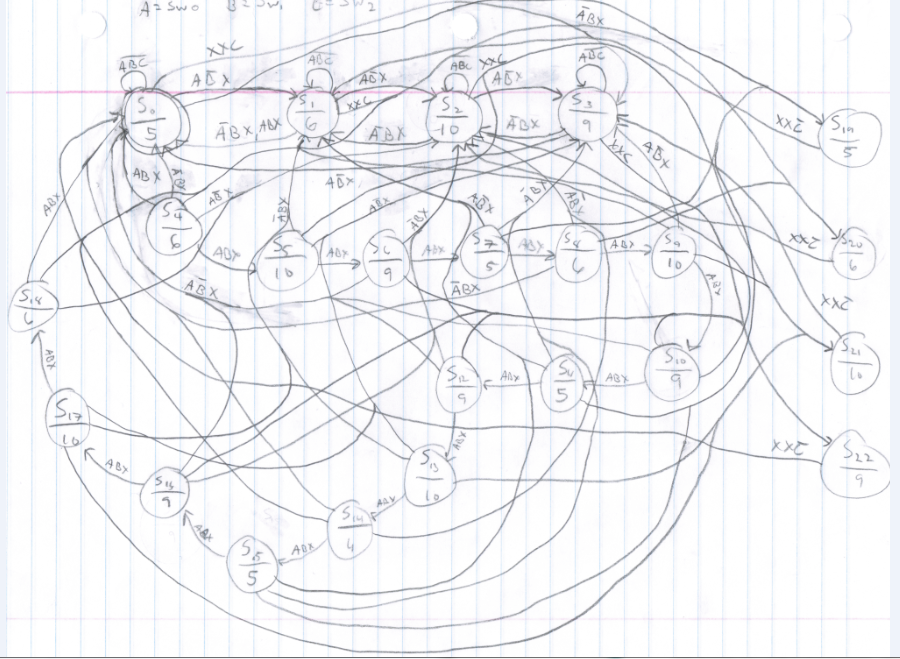
\includegraphics[width=\textwidth]{FSM_compress}}
%FSM here

\subsubsection*{Scope}
Phase 1 is the preparation; phase 2 is the demonstration; and phase 3 is the lab report. 

\subsubsection*{Prototypes}
A prototype system running on the LM3S1968 board and solderless breadboard will be demonstrated. Progress will be judged by the preparation, demonstration and lab report.
\subsubsection*{Performance}
The system will be judged by three qualitative measures. First, the software modules must be easy to understand and well-organized. Second, the system must employ a finite state machine running in the background. There should be a clear and obvious abstraction, separating what the machine does (the FSM state diagram) from how the machine works (the software ISR). Backward jumps in the ISR are not allowed. Third, all software will be judged according to style guidelines. Software must follow the style described in Section 3.3 of the book. There are three quantitative measures. First, the speed of oscillations will be measured, with an attempt to make it oscillate as fast as possible. Second, the maximum time to run one instance of the ISR will be recorded. Third, you will measure power supply current to run the system. There is no particular need to minimize current in this system.
\subsubsection*{Usability} 
There will be three switch inputs. The stepper motor will operate under no load conditions, 2.6. Safety: Explain any safety requirements and how they will be measured. Stepper motors draw current even when not moving. For simple edit compile download changes you can leave the motor powered. However, for longer edit sessions, disconnect the +5V power to the motor. For example, when developing software that does not involve the motor: 1) Disconnect the USB cable; 2) Disconnect the +5V power to the protoboard/motor; 3) Reconnect the USB cable; 4) Edit/debug software. When developing software that does involve the motor: 1) Disconnect the USB cable; 2) Edit and compile software; 3) Reconnect the USB cable; 4) Download/debug software. Connecting or disconnecting wires on the protoboard while power is applied may damage the board.
\subsection*{Deliverables}
\subsubsection*{Reports}
A lab report described below is due by the due date listed in the syllabus. This report includes the final requirements document.
\subsubsection*{Audits}
The preparation is due at the beginning of the lab period on the date listed in the syllabus.
\subsubsection*{Outcome}
There are three deliverables: preparation, demonstration, and report.

\section*{Measurement Data}
\begin{enumerate}
\item System Power: 
\subitem Voltage: 5v 
\subitem Current: 340mA without motor running, 316mA with motor driving.
\item Motor Rate: About 3000 $\mu$seconds. 334 Hz or about 14 revolutions a second. This is nearing the fastest rate that the inductors can switch.
\item ISR Execution Time: 19.7 $\mu$seconds.\\
\centerline{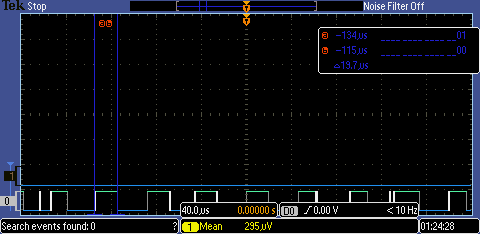
\includegraphics[width=1\textwidth]{TEK00000}}
\end{enumerate}

\section*{Analysis and Discussion}
\begin{pset}
  \problem{1}
  What is jerk? How is it minimized?
  \emph{Jerk is the derivative of accelartion. It is seen as non smooth or jerky motion, and can be minimized by slowing large changes in acceleration.}
  \problem{2}
  Draw an electrical circuit model for one stepper motor coil, and explain the components
  \vskip 0.25in
\centerline{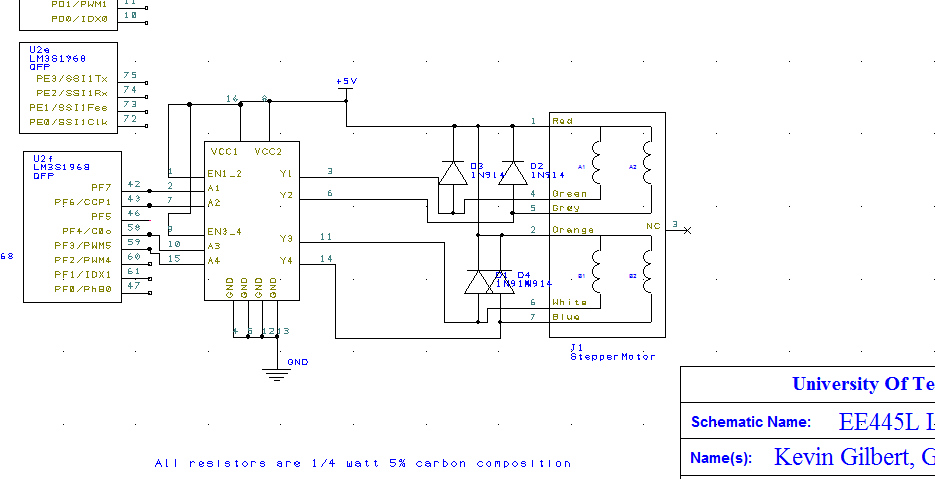
\includegraphics[width=1\textwidth]{stepper}}
  \vskip 0.1in
  \emph{The stepper motor operates by using a set of inductors as electro magnets in series. When one is turned on, the rest are disabled. The pulls the closest internal cog on the motor shaft to the magnet. When that magnet is disabled and the next one enabled, the shaft is rotated again. This provides fine control of the motor output.}
  \problem{3}
  Explain what parameters were important for choosing a motor drive interface chip (e.g., L293 or 2N2222). How does your circuit satisfy these parameters?\\
  \emph{Voltage input, output and current driving capabilities are highly important when deciding on a motor interface chip. If the interface device cannot supply enough current to the motor, or under/over supplies the device with voltage, then at best case the device will do nothing, or in the worse case damage a component. The L293 fits our requirements for the stepper motor being used. The chip runs off of 5 volts, and can supply up to an amp of current.}
  \problem{4}
  What happens to the current when a mechanical load is applied to the shaft? Why? \\
  \emph{Current draw on a motor is dependent on the load applied. Beyond the base amperage required to overcome stiction and the resistance of the device, more current is used when resistance is added to the output.}
  \problem{5}
  If the motor is spinning at a constant rate, give a definition of electrical power in terms of parameters of this lab. Research mechanical power. Give a definition of mechanical power. Are the two related? \\
  \emph{Electrical power is defined as the voltage times current draw. Mechanical power is defined as the product between force appplied to the shaft and angular velocity. This maps to the electrical properties of a DC motor. The voltage controls the motor's speed, while current is dependent on the force applied to the shaft.}
\end{pset}

\end{document}